\documentclass[12pt, openany]{report}
\usepackage[utf8]{inputenc}
\usepackage[T1]{fontenc}
\usepackage[a4paper,left=2cm,right=2cm,top=1cm,bottom=2cm]{geometry}
\usepackage[french]{babel}
\usepackage{libertine}
\usepackage[pdftex]{graphicx}
\usepackage[export]{adjustbox}
\usepackage{setspace}
\usepackage{hyperref}
\usepackage{enumitem}
\usepackage[nottoc]{tocbibind}
\usepackage{amsmath,diagbox,tabu}

\hypersetup{
    colorlinks=true,
    linkcolor=black,
    filecolor=magenta,      
    urlcolor=cyan,
}
\setstretch{1,4}
\setlength{\parindent}{4ex}
\setlength{\parskip}{1ex plus 0.5ex minus 0.2ex}
\newcommand{\hsp}{\hspace{20pt}}
\newcommand{\HRule}{\rule{\linewidth}{0.5mm}}

\newlist{mylist}{itemize}{3}
\setlist[mylist,1]{
    label=\textbullet,
    wide=0pt,
    itemindent=\dimexpr\parindent+\labelwidth+\labelsep\relax}

\begin{document}
\begin{titlepage}
  \begin{sffamily}
  \begin{center}

	\begin{figure}[t]
	   \begin{minipage}{0.48\textwidth } 
	     
\includegraphics[width=.3\linewidth , left]{ensias.JPG}
	   \end{minipage}\hfill
	   \begin{minipage}{0.48\textwidth }
	     
\includegraphics[width=.4\linewidth , right]{univesite.JPG}
	   \end{minipage}
	\end{figure}
     
    \textsc{\LARGE École nationale supérieure d'informatique et d'analyse des systèmes}\\[4cm]


    % Title
    \HRule \\[0.5cm]
    { \huge \bfseries Présentation du sujet de projet de fin d'année: Crop Mapping\\[0.4cm] }
	\HRule\\[4cm]

    % Author and supervisor
    \begin{minipage}{0.4\textwidth}
      \begin{flushleft} \large
        \emph{Réalisé par:}\\
            AIT LAHCEN \textsc{Ahmed}\\
	        CHICHI \textsc{Hamza}\\
       \emph{Filière, Groupe}\\
	        Génie logiciel, GL 1\\
      \end{flushleft}
    \end{minipage}
    \begin{minipage}{0.4\textwidth}
      \begin{flushright} \large
       \emph{Sous la direction de:}\\
	Mme. Sanaa. \textsc{EL FKIHI}\\
	\end{flushright}
    \end{minipage}

    \vfill

    % Bottom of the page
    {\large Année universitaire 2019/2020}

  \end{center}
  \end{sffamily}
\end{titlepage}
\newpage
\strut 


\listoffigures
\tableofcontents
\chapter*{Introduction générale}
\addcontentsline{toc}{chapter}{Introduction générale}

Le domaine de l’agriculture constitue une grande partie économique de plusieurs pays dans le monde, ce qui rend la recherche scientifique envers ce secteur d’activité une importante source de revenue financier, mais ceci n’est possible que si la disponibilité des ressources de l’environnement biophysique et humain est importante.
\par
En effet, l’exploitation des images satellites sur les terrains agricoles permet de gérer plus efficacement les récoltes et de prévoir les risques pouvant menacer la production comme par exemple les risques d’infestations d’insectes, les intempéries, la sécheresse ... Et ceci grâce aux différents caractéristiques contenues dans une image satellitaire (longueurs d’ondes, fréquences, domaines spéctraux..)
\par
Si l’agriculture représente un secteur économique très important pour un pays, comme le Maroc par exemple, vaut mieux investir dans la recherche de nouvelles technologies dans ce domaine afin d’exploiter au maximum ses ressources, sans oublier que le développement de l’agriculture moderne ne cesse d’accroitre et que certains pays se sont mis à l’introduction dans les pratiques agricoles de nouveaux outils numériques d’aide à la décision basés sur le monde de la big data et des nouvelles technologies (drones, robots…).
\par
Parmi les technologies modernes qui facilitent la tâche pour les acteurs de la production et augmente la consommation	 agricole, on retrouve le \textbf{Crop Mapping}, qui est le sujet de notre projet de fin d’année.  Cette dernière est une techniques qui utilise des données fournies par les image satellites pour les analysées et les traitées en utilisant plusieurs méthodes telles que le Deep Learning et le réseaux de neurones afin d’élaborer des stratégies pour les champs et les cultures pour le long terme.
\par
Ce rapport est constitué en deux parties. La première partie, intitulée contexte générale du projet, comporte ... chapitres, le premier présente les notions générales du sujets.


\chapter{Présentation du sujet}
Cette partie va présenter les différentes notions abordées dans le projet accompagnées de quelques exemples. 

\section{Les parcelles}

\subsection{Définition de parcelle}
Une parcelle est généralement une superficie de terrain ayant une unité de propriété, elle peut être dans ce cas la propriété privée ou publique d'une personne ou d'un groupe.\\
Un ensemble de parcelles peut être désigné comme un « parcellaire ». 

\begin{figure}[hp]
\centering
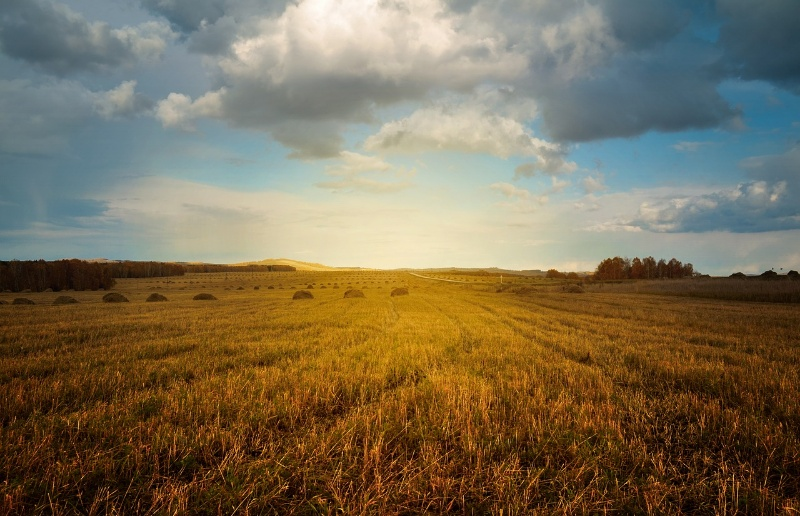
\includegraphics[scale=0.4]{parcelle2.jpg}
\caption{Une parcelle}
\end{figure}


Le terme de parcelle peut s'appliquer à différents domaine :

\begin{mylist}

\item En agriculture, elle désigne la division agricole (champ, pré, vignoble, verger, etc.) exploitée par la même personne ou le même groupe de personnes.


\item En urbanisme, elles sont définies selon leurs propriétaires et leurs limites, tant en milieu rural qu'urbain. Ainsi elle peut être un terrain habité, ou encore une parcelle à l'abandon ou bien une zone de stationnements automobiles. 

\end{mylist}



\subsection{La segmentation des parcelles}

La fragmentation spatiale des parcelles agricoles a un fort impact sur les flux d’eau dans les paysages cultivés, et pour surveiller les paysages à grandes échelles, il y a un fort besoin de délimitation automatique ou semi-automatique des parcelles agricoles. C’est pour cela que la contribution des images satellitaires à très haute résolution peut permettre la délimitation en utilisant de nombreuses méthodes de classification et des algorithmes qui traitent les caractéristiques de ces images.\cite{frag}

\begin{figure}[hp]
\centering
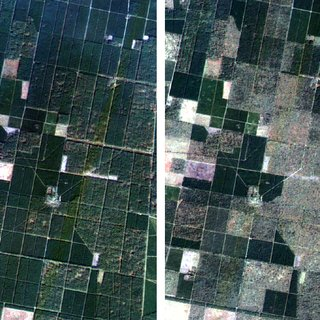
\includegraphics[scale=1]{seg.jpg}
\caption{La fragmentation d'une parcelle}
\end{figure}

Le résultat de ces études permet une bonne localisation des limites parcellaires et met en évidence l’intérêt d’un modèle global si une base de données d’images de limites parcellaires existe. 

\newpage

\subsection{L'agriculture au Maroc}

L'agriculture est un secteur économique très important du Maroc. Il génère environ 14 \% du produit intérieur brut (PIB), mais avec des variations importantes (11 à 18 \%) selon les années en fonction des conditions climatiques. Ses performances conditionnent même celles de l’économie tout entière : le taux de croissance du pays est fortement corrélé à celui de la production agricole. L’agriculture demeure par ailleurs le premier pourvoyeur d’emplois du pays, loin devant les autres secteurs économiques, 40 \% de la population active vivant de ce secteur.\cite{imagesatt}


\begin{figure}[hp]
\centering
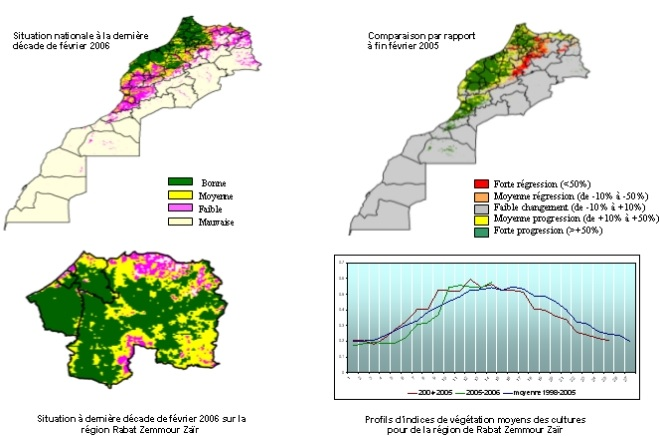
\includegraphics[scale=0.8]{etat.jpg}
\caption{L'état des cultures au maroc}
\end{figure}


Les principales productions végétales du pays sont constituées par les céréales (blé, orge), les agrumes (oranges, clémentines), les olives, les rosacées fruitières (amandes, pommes, abricots...), les betteraves à sucre, les légumineuses alimentaires, les cultures maraichères dont les pommes de terre et les tomates, fer de lance des exportations agricoles marocaines. L'élevage (ovin, caprin, bovin, camelin, avicole) constitue aussi une composante importante du secteur agricole en contribuant à hauteur de 30 \% à sa valeur ajoutée.

\section{Les images satellites}
Un satellite artificiel est un objet fabriqué par l'être humain, envoyé dans l'espace à l'aide d'un lanceur et gravitant autour d'une planète ou d'un satellite naturel comme la Lune.  
Le premier satellite artificiel Spoutnik 1 est lancé par l’Union des républiques socialistes soviétiques en 1957.
\subsection{Les sattelites en orbite autour de la terre}


Selon l'association UCS (Union of Concerned Scientists), 2.063 satellites opérationnels étaient en orbite autour de la Terre au 1er avril 2019. Le plus ancien encore en opération est un satellite amateur américain, Amsat-Oscar 7 (AO-7), lancé le 15 novembre 1974. La cadence des lancements s'est brusquement accélérée ces dernières années, avec 378 satellites lancés en 2017 et 375 satellites en 2018. Attention : il ne s'agit pas du nombre de fusées, car les lancements multiples sont devenus la norme. Le 15 février 2017, l'Inde a ainsi battu un record avec 104 satellites en un seul tir.\cite{orbite}

\begin{figure}[hp]
\centering
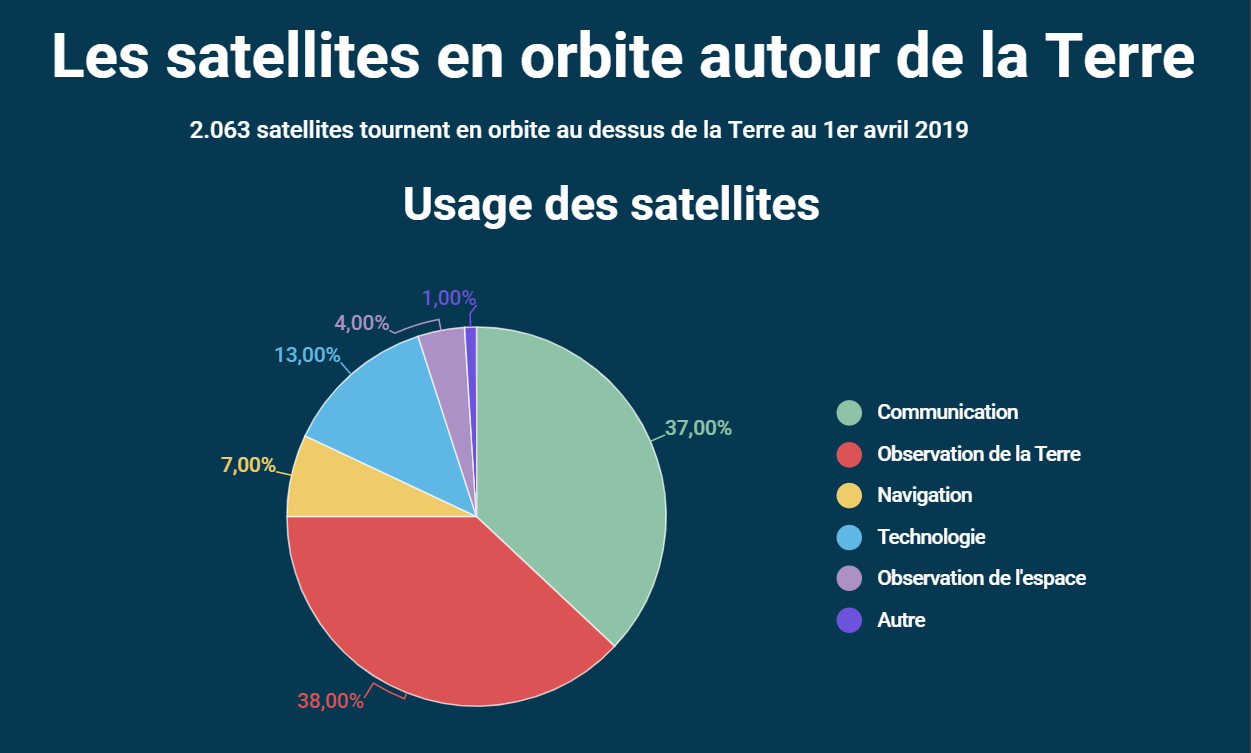
\includegraphics[scale=0.6]{satellite.png}
\caption{Statistiques de satellites}
\end{figure}

\subsection{Les satellites marocains}
Mohammed VI est un système de 2 satellites de reconnaissance et d'observation de la Terre (A et B) du type Pléiades, conçu par Thales Alenia Space (conception de la charge) et Airbus (conception de la plate-forme satellitaire) pour le compte du Centre royal de télédétection spatiale (Maroc).
\par
Le satellite Mohammed VI A est lancé le 8 novembre 2017 par un lanceur Vega depuis le Centre spatial de Kourou satellite espion, il est utilisé pour surveiller le Front Polisario dans la « zone tampon ».
Le lancement du deuxième satellite (Mohammed VI B) est effectué avec succès le 21 novembre 2018, à usage civil, est utilisé pour la cartographie et le cadastre, l’identification des zones sinistrées...
\begin{figure}[h]
\centering
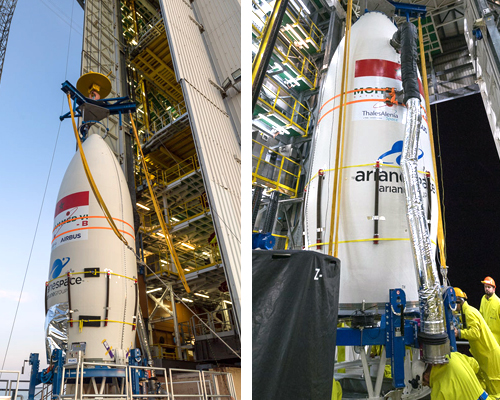
\includegraphics[scale=0.8]{satm6.jpg}
\caption{Le satellite MOHAMMED VI - B}
\end{figure}


\subsection{La définition d'une image satellite}
Une image satellite, ou image satellitaire, est une prise de vue transmise d'un satellite artificiel en orbite. Elles permettent d'obtenir différentes informations comme la surveillance des pays ennemis pour les militaires (fonction première de la création d'un satellite d'observation), prévisions météorologiques (par exemple les satellites Météosat), ou tout simplement pour les recherches sur l'Univers. Certains satellites sont capables d'une précision telle que cela peut devenir un problème, notamment en termes de vie privée ou de secret d'État. 

\subsection{Les caractéristiques des images satellites}
La principale différence entre une photographie et une image satellite est que la photographie est au format analogique et qu’elle est généralement imprimée sur papier avant d’être interprétée. L’image satellite est au format numérique et elle est généralement analysée et interprétée à l’aide d’un ordinateur.Le format numérique enregistre chaque bloc d’informations de manière discrète.


\par
\underline{Le pixel :}
\par

Avec un zoom avant suffisant sur une image satellite, on peut voir de nombreux carrés de couleurs différentes qui sont les pixels.
Ces pixels représente la plus petite unité figurant sur une image. Réunis, ils fournissent toute l’information qui constitue l’image dans son intégralité.

\par
\underline{La résolution spatiale :}
\par 

La résolution spatiale d’une image est la plus petite distance entre deux objets adjacents que le capteur puisse identifier.
Plus les pixels seront nombreux dans l’image plus la résolution spatiale sera élevée.
\par
Selon les caractéristiques du capteur, l’altitude du satellite ,son orbite autour de la Terre, les images satellites seront composées de pixels couvrant une surface au sol plus ou moins grande du sol. On classera ainsi les images enregistrées en images : Basse , moyenne, haute résolution ou très haute résolution.

\begin{figure}[h]
\centering
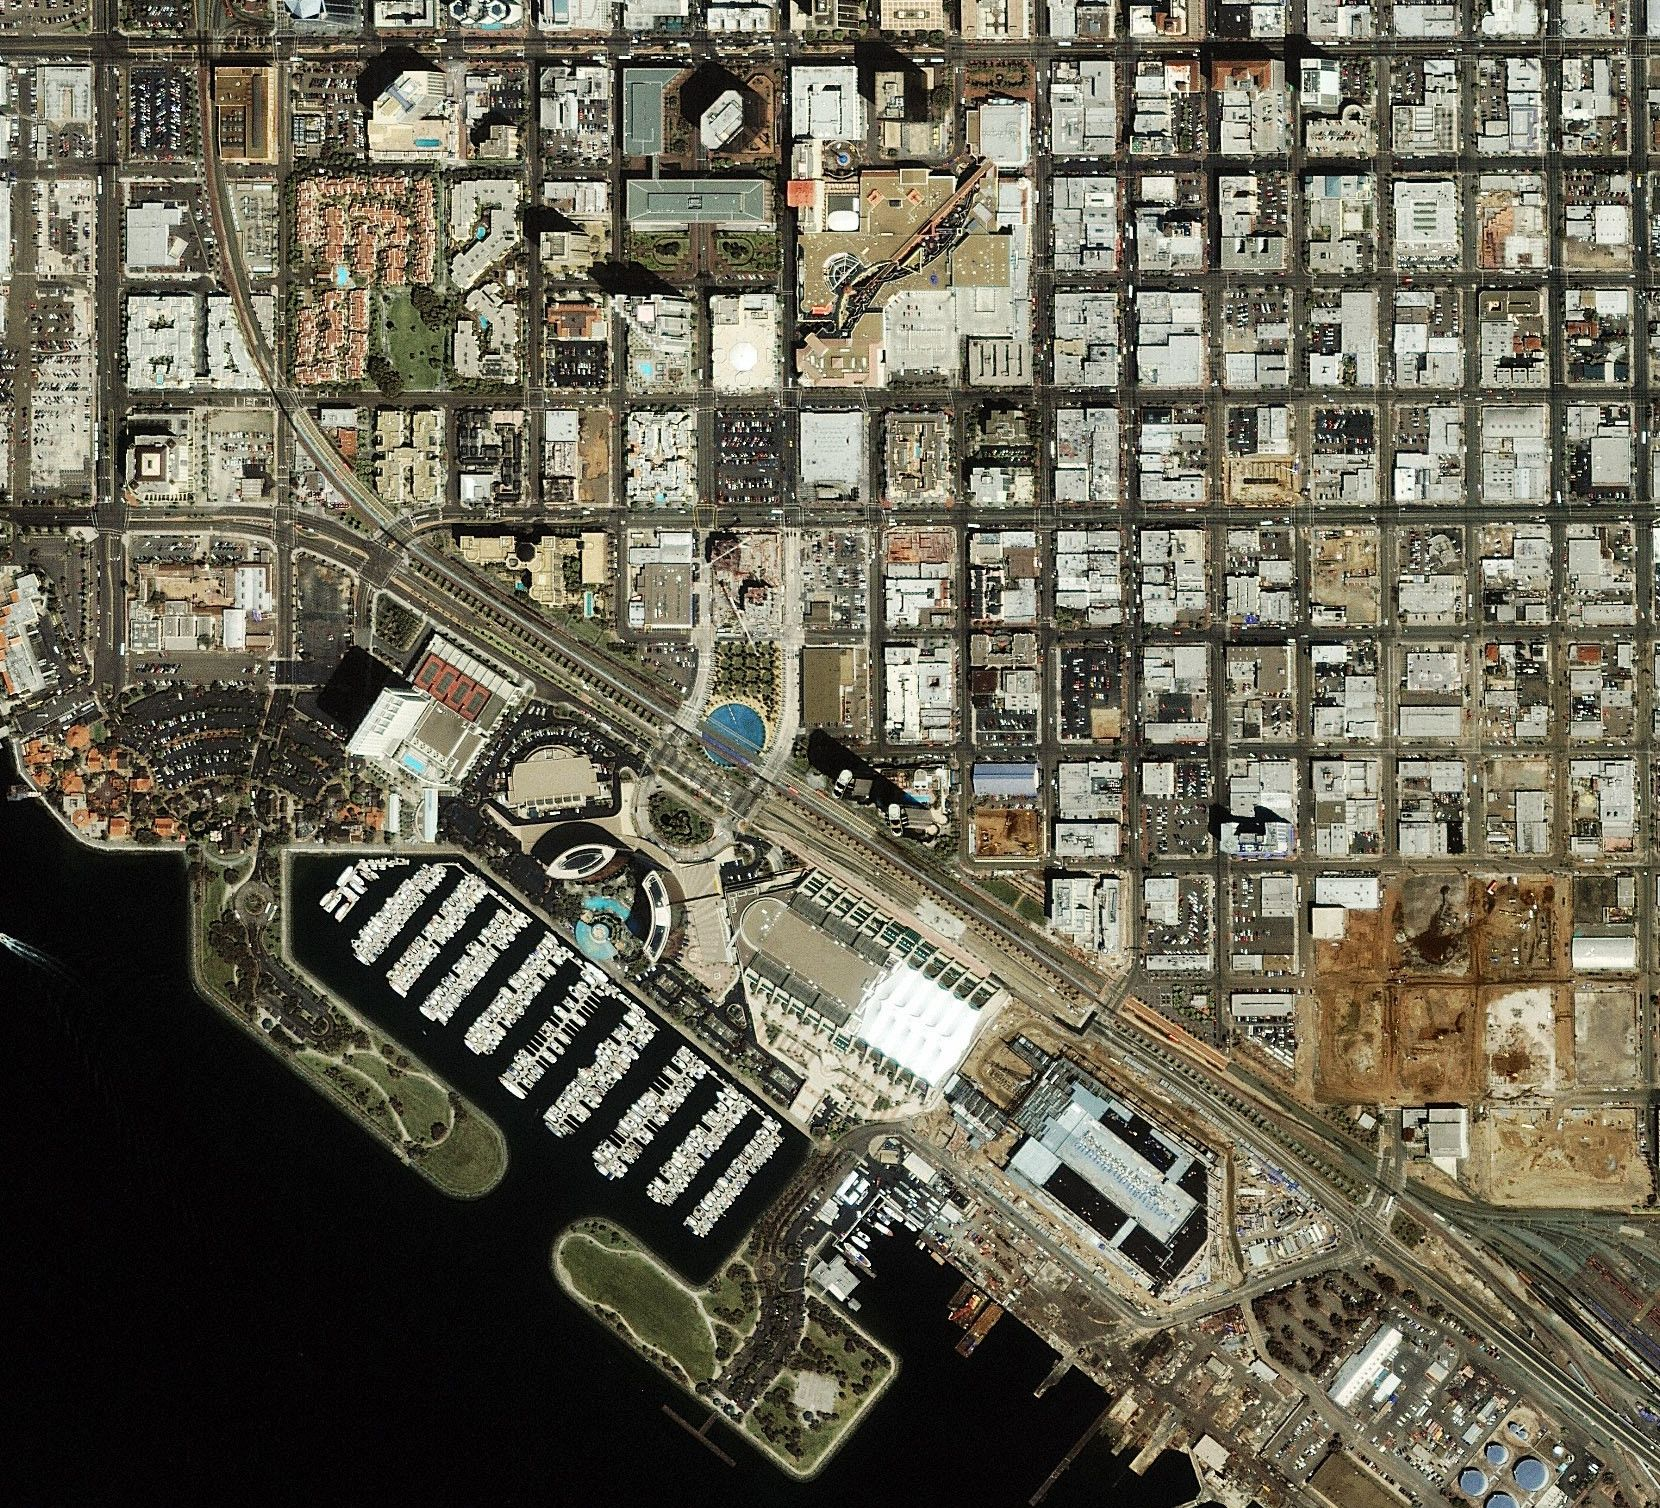
\includegraphics[scale=0.25]{resolution_image.jpg}
\caption{Image satellite en très haute résolution}
\end{figure}

\par
\underline{Valeur des pixels :}
\par 

Chaque pixel d’une image a une valeur. Cette valeur correspond à l’intensité du rayonnement réfléchi par l’objet observé dans la gamme de longueur d’ondes auxquelles le capteur est sensible. \cite{ref3}

La valeur du pixel varie de 0 (= noir) à 255 (= blanc). Donc, il y a 256 possibilités, ce qui correspond à 1 octet. Cela représente la quantité de rayonnement détectée par un capteur, allant du minimum au maximum. Le nombre de niveaux donne une indication quant à la précision de la mesure : plus il y a de niveaux (donc plus il y a de bits), plus détaillée sera la mesure et donc plus précise sera la mesure de la variation du rayonnement.

\begin{figure}[h]
\centering
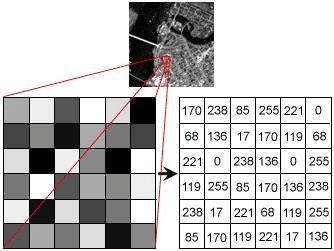
\includegraphics[scale=1.2]{pixel_values.png}
\caption{Les valeurs des pixels}
\end{figure}

\par
En observation de la Terre on peut exploiter :
\begin{mylist}
\item
des ondes émises par le soleil puis réfléchies par la surface de la Terre et enregistrées par un capteur placé sur un satellite.
\item
des ondes émises par un émetteur artificiel placé sur le satellite puis réfléchies par la surface de la Terre et enregistrées par un capteur placé sur ce même satellite.
\end{mylist}

Dans le premier cas on parle d'\textbf{images optiques} (télédétection passive), dans le second cas d'\textbf{images radar} (télédétection active).

\begin{figure}[h]
\centering
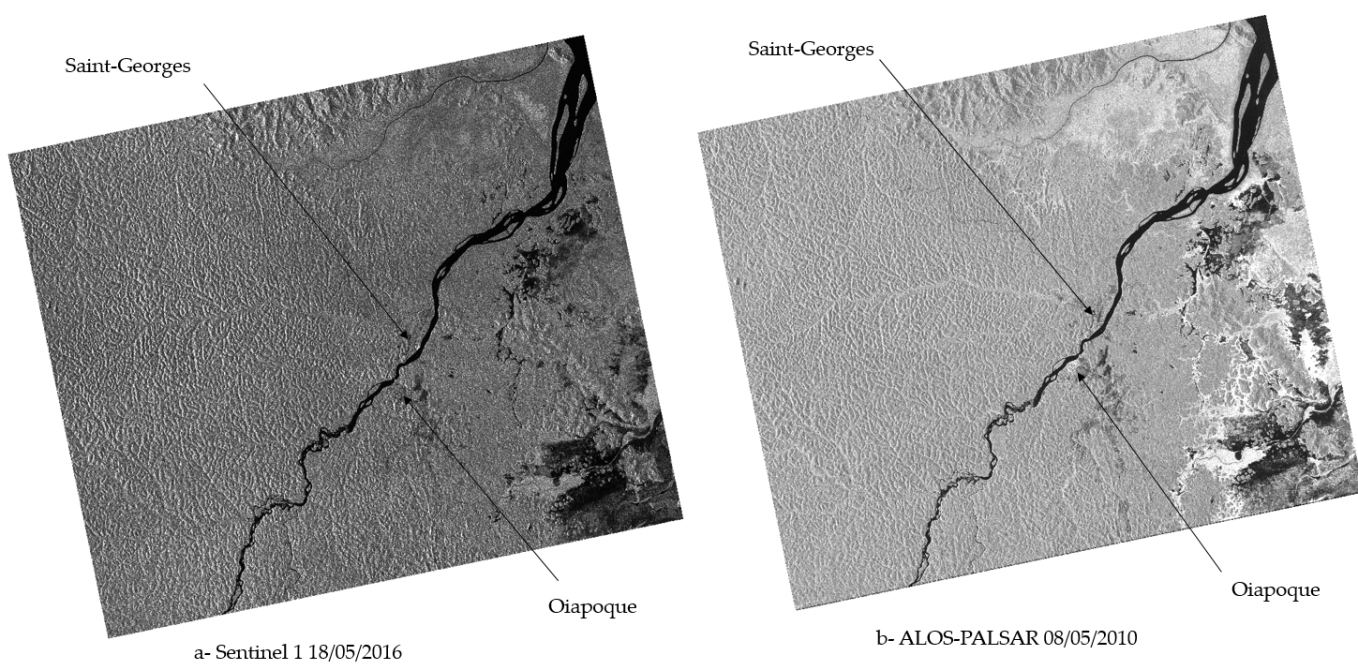
\includegraphics[scale=0.3]{image_radar.png}
\caption{Exemple d'image radar prise par le sattellite Sentinel-1 et ALOS/PALSAR}
\end{figure}

\par
La télédétection radar présente l’avantage de s’affranchir des contraintes de couverture nuageuse : les ondes émises par les satellites traversent les nuages pouvoir acquérir des images de jour comme de nuit. En revanche, leur exploitation pour l’observation de la Terre est moins intuitive quel les images optique, ainsi différents domaines spectraux sont exploité (longueurs d’onde du visible à l’infrarouge).\cite{ref4} \\ \\ \\



\subsection{Les satellites au service de l'agriculture}

Dans le domaine de l'agriculture, les satellites d'observation de la Terre sont utilisés pour une très grande variété d’applications et de services, comme la surveillance des cultures, le contrôle des surfaces et de l'occupation des sols, l'irrigation et la des gestion des cultures en engrais et produits phytosanitaires. Ils sont également utilisés pour suivre la production d'herbe tout au long de la saison culturale.  \cite{satt}


\begin{figure}[h]
\centering
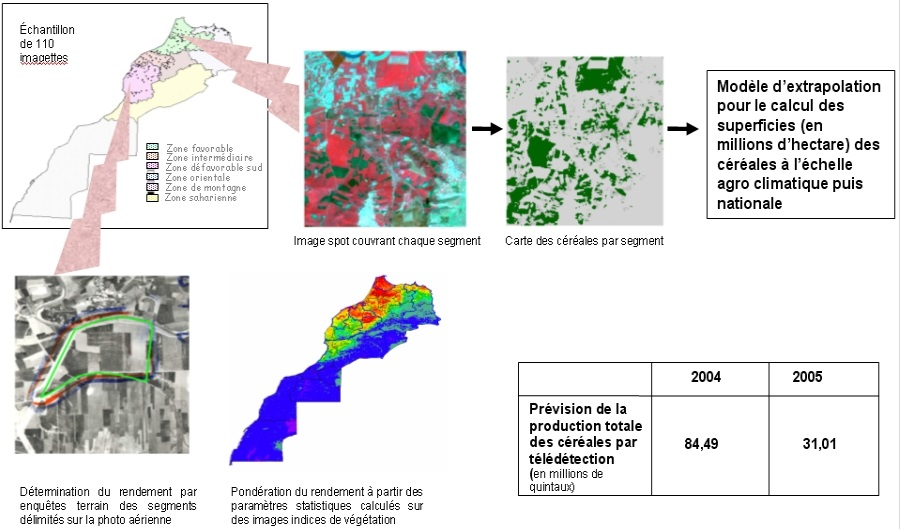
\includegraphics[scale=0.65]{prev.jpg}
\caption{Prévision de la production des céréales à l'échelle nationale}
\end{figure}

L'intérêt d'utiliser des satellites s'explique par leur capacité à  fournir des images multi spectrales de très bonne résolution. Ces images reçues dans plusieurs longueurs d'onde permettent d'estimer des paramètres biophysiques à partir des pixels de l'image que l'on mesure dans plusieurs couleurs de façon à caractériser l'état de la plante.
\par
Ce type d'image a supplanté les systèmes antérieurs en démontrant qu'il pouvait prendre en compte l'état réel des cultures et de la croissance de la végétation à l'intérieur des parcelles à différents stades de la pousse.

\section{Crop Mapping}
\subsection{Définition}
C’est une technique en agriculture qui utilise des données GPS pour analyser des variables telles que le rendement des cultures et la teneur en eau dans un champ donné. Il a été développé dans les années 1990 et utilise une combinaison de technologie GPS et de capteurs physiques, tels que des compteurs de vitesse , pour suivre les rendements des cultures, la vitesse de l'élévateur à grains et combiner la vitesse.
\par
Ces données produisent une carte des rendements qui peut être utilisée pour comparer la distribution des rendements dans le champ d'une année à l'autre. Cela permet aux agriculteurs de déterminer les zones du champ qui, par exemple, peuvent avoir besoin d'être plus fortement irriguées ou qui ne produisent aucune récolte. Il permet également aux agriculteurs de montrer les effets d'un changement dans les techniques de gestion des champs, d'élaborer des stratégies nutritionnelles pour leurs champs et d'enregistrer le rendement des cultures à utiliser pour obtenir des prêts ou des locataires.

\subsection{Les méthodes de Crop Mapping}

Il y a plusieurs méthodes de Crop Mapping dont:

\subsubsection{La télédétection (remote sensing from space)}
La télédétection offre une méthode sûre et efficace de cueillette d'information dans le but de cartographier le type et de calculer la superficie des cultures.
Les micro-ondes sont sensibles à l'alignement, la structure et la quantité d'eau présente dans les plantes et dans le sol, et peuvent fournir de l'information complémentaire aux données optiques. 

\par
Les résultats de l'interprétation des données de télédétection peuvent être intégrés dans un système d'information géographique (SIG) et dans un système de gestion des cultures, et peuvent aussi être combinés à des données auxiliaires pour fournir de l'information sur les droits de propriété, les pratiques de gestion, etc. \cite{cropmapp}\\ \\ \\

\begin{figure}[h]
\centering
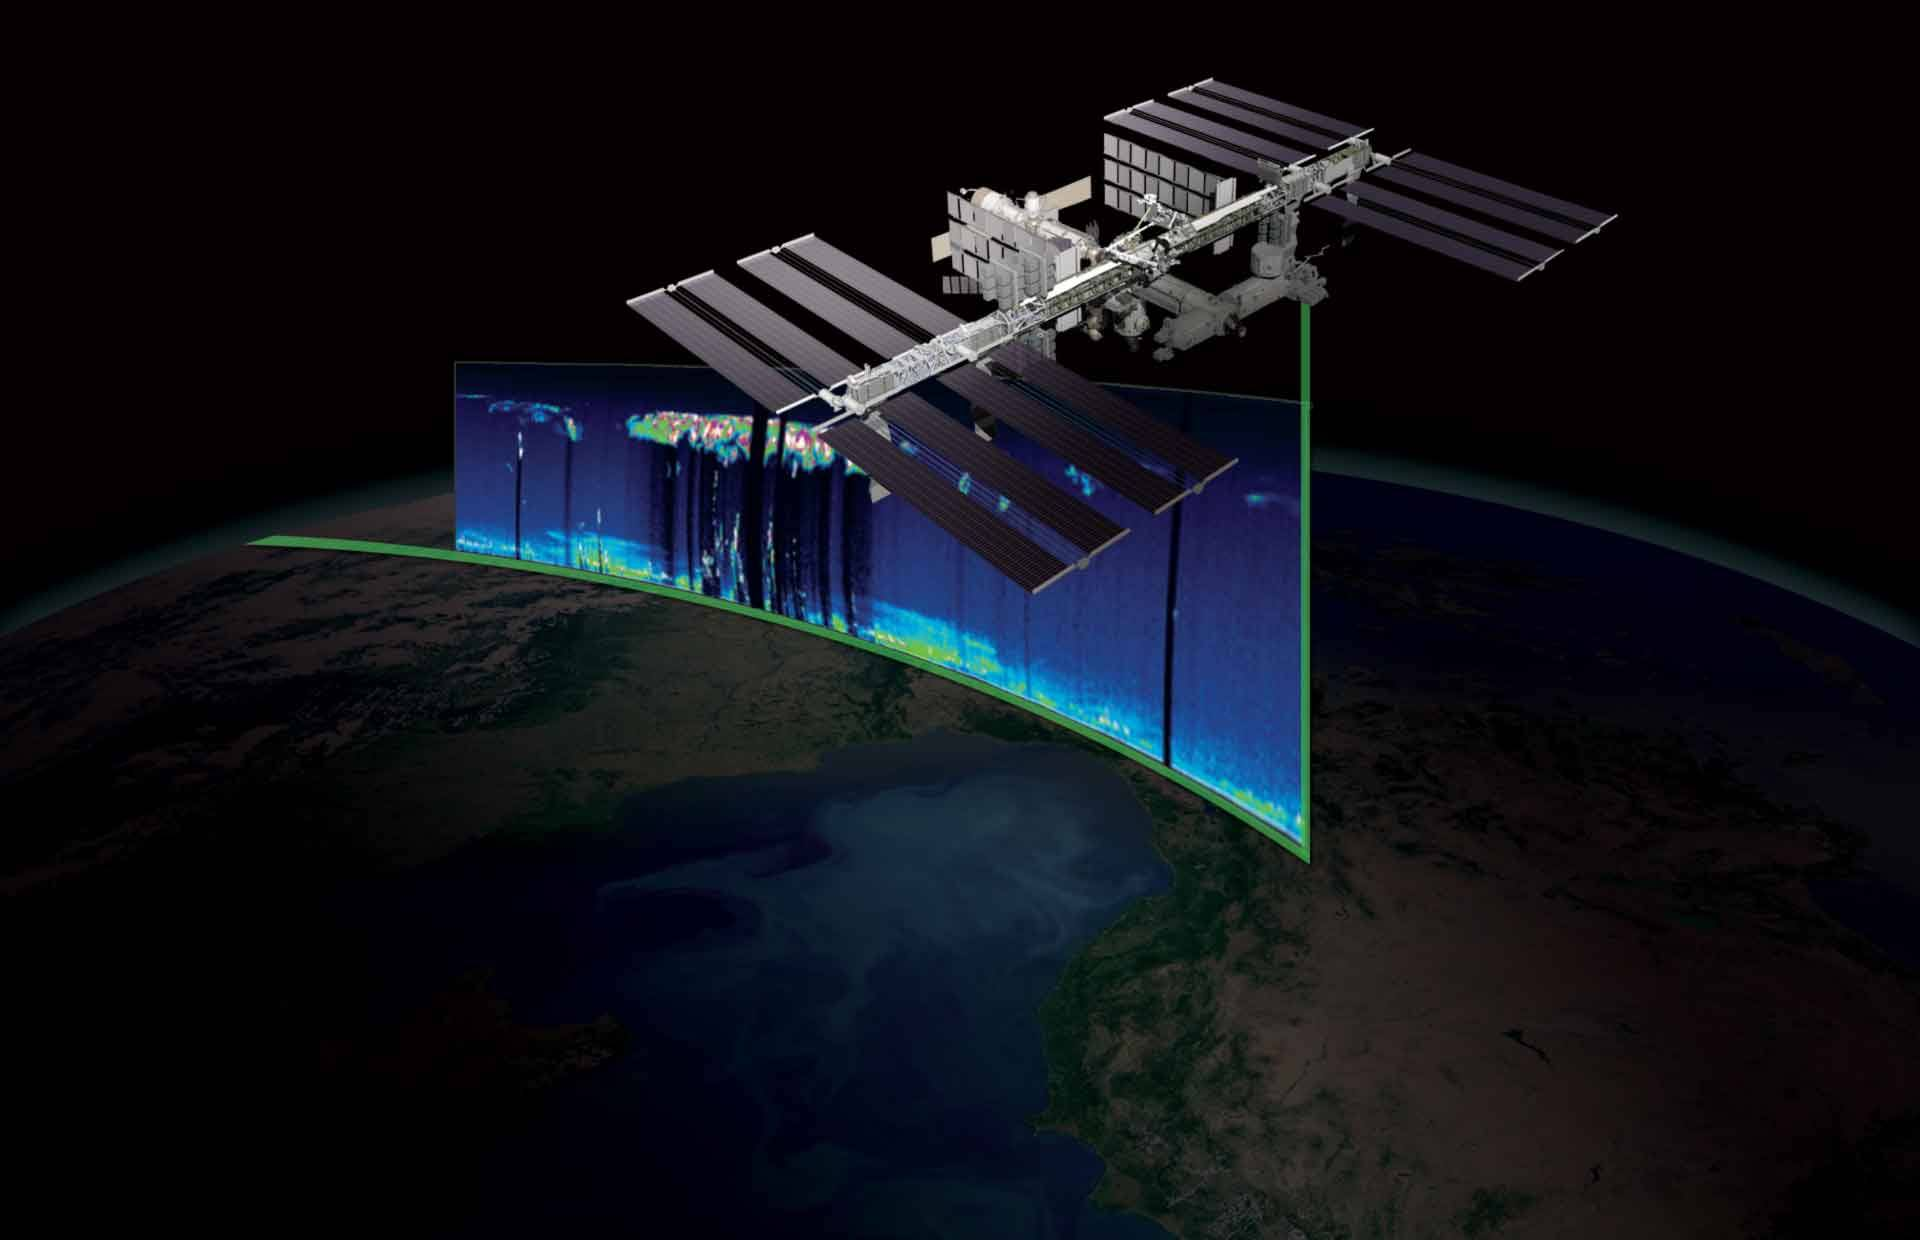
\includegraphics[scale=0.2]{tele.jpg}
\caption{La télédétection par satellite}
\end{figure}

\subsubsection{MODIS (Moderate Resolution Imaging Spectroradiometer)}
MODIS est un instrument clé à bord des satellites Terra et Aqua qui sont en orbite de la terre et qui visualise la totalité de sa surface tous les 1 à 2 jours, acquérant des données dans 36 bandes spectrales.

\begin{figure}[h]
\centering
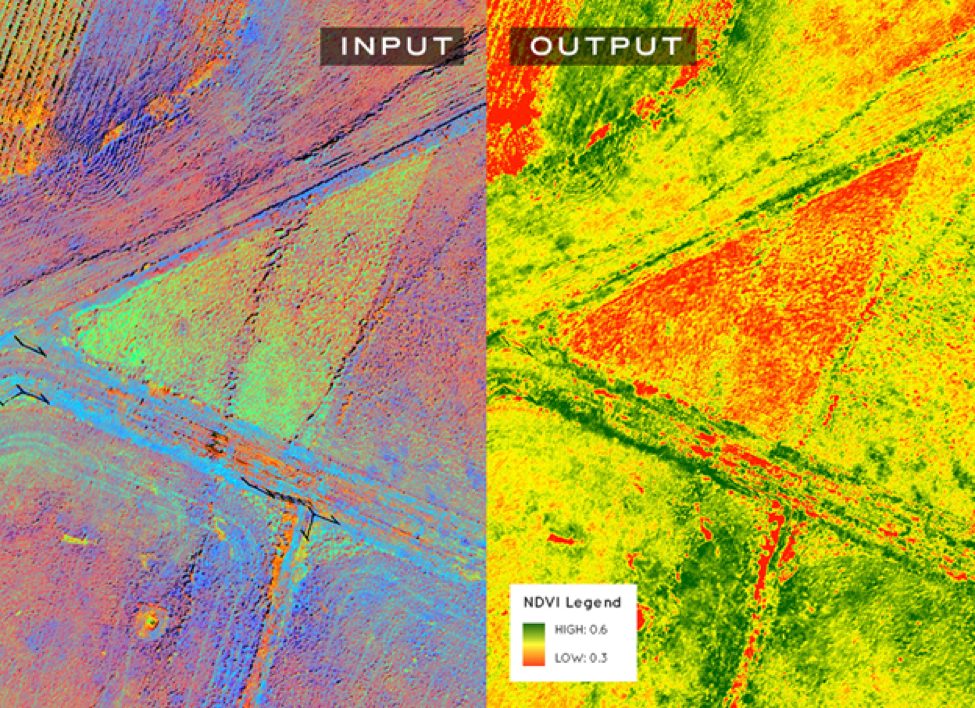
\includegraphics[scale=0.35]{modis.png}
\caption{Une comparaison Input/Output par la méthode MODIS}
\end{figure}

MODIS présente deux indices de végétation (NDVI et EVI) qui fournissent des comparaisons spatiales et temporelles des différentes surfaces à couvert végétale et foliaire, le NDVI (normalized difference vegetation index) assure la continuité de la série temporelle pour des applications historiques et climatiques tandis que le EVI minimise les variations de la canopée et améliore la sensibilité aux conditions de végétation dense.
Ces deux indices caractérisent plus efficacement la gamme mondiale des états et des processus de végétation. \cite{modis}

\subsubsection{Deep Learning Classification}
Le Deep Learning (DL) est une technique de pointe puissante pour le traitement d'image, y compris les images de télédétection (remote sensing images). 
Pour cibler la couverture des sols et la classification des types de cultures à partir d'images satellites multi-temporelles et multi-sources, une architecture DL à plusieurs niveaux solide doit être disposer. 
Le pilier de cette architecture est un réseau neuronal qui est utilisé pour la segmentation des images optiques et la restauration des données manquantes en raison des nuages et des ombres. \cite{deeplearning}

L’avantage de cette méthode est d’étudier des modèles de deep learning/machine learning pour la « crop classification » qui fournissent une segmentation basée sur les pixels d'une zone d'inspection pendant une période donnée. Pour obtenir de meilleurs résultats, il est préférable d’utiliser des modèles existant et de sélectionner ceux les mieux adaptés à la situation. Et pour mieux de flexibilité, il faut ajuster les modèles pré-formés par transfert learning à de nouvelles données comme de nouveaux domaines avec de nouvelles particularités, cultures...

Un autre avantage est le potentiel d'améliorer considérablement la précision d'un modèle avec plus de données réelles recueillies au sol de la région étudié en utilisant des données spécifiques. Cependant, il est possible d'obtenir de meilleurs résultats avec l'ensemble de données de formation (training data set) plus spécifiques.

\begin{figure}[h]
\centering
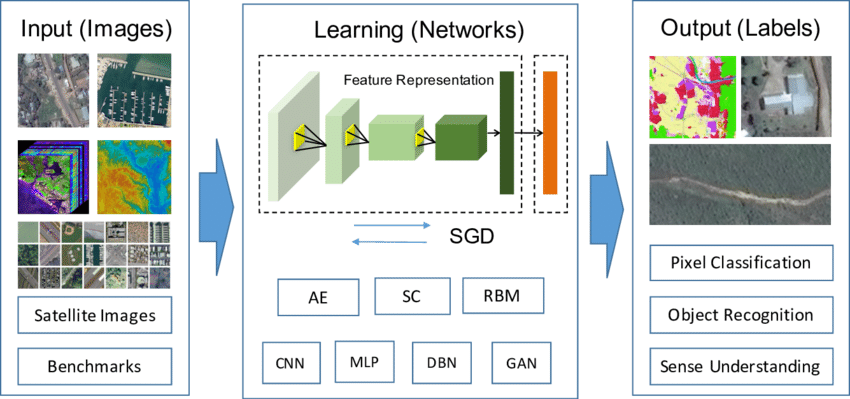
\includegraphics[scale=0.5]{deep.png}
\caption{Le processus de Deep Learning}
\end{figure}

\subsection{Outils pour le Crop Mapping}

On a essayé de faire une comparaison entre les outils les plus populaires dans le domaine du Crop Mapping :

{\setlength{\tabulinesep}{3pt}
\begin{tabu}{|c|c|c|c|c|c|}
\hline
\diagbox{caractéristiques}{L'outil} & ENVI & QGIS & ArcGIS & CMaps Analytics & TerrSet\\
\hline
Imagerie 3D & - & + & + & - & -\\
\hline
Intégration des données du recensement & - & + & + & + & -\\
\hline
Géocodage & - & + & + & + & +\\
\hline
Exportation d'images & + & + & + & - & +\\
\hline
Cartographie Internet & + & - & + & + & -\\
\hline
L'interopérabilité & - & + & + & + & -\\
\hline
Étiquetage & + & + & + & - & -\\
\hline
Création de carte & + & + & + & + & +\\
\hline
Partage de carte & - & - & + & + & -\\
\hline
Analyse spatiale & - & + & + & + & +\\
\hline
\end{tabu}}

\begin{thebibliography}{9}

\bibitem{frag}
Agriculture et Biodiversité en Bretagne\\
\textit{Freagmentation du parcellaire}. \\
\url{http://www.agriculturebiodiversite.fr/ameliorer-la-biodiversite/amenager-son-exploitation/fragmentation-du-parcellaire.html}

\bibitem{imagesatt}
Les images et les statistiques concernat le Maroc\\
\textit{Centre Royal de Télédétection Spatiale}.\\
\url{https://www.crts.gov.ma/thematiques/agriculture/suivi-d-etat-des-cultures}

\bibitem{orbite}
Combien de satellite tournent autour de la Terre ?\\
\textit{Céline Deluzarche, Publié le 12/04/2020, FUTURA SCIENCES}\\
\url{https://www.futura-sciences.com/sciences/questions-reponses/satellite-satellites-tournent-autour-terre-7065/}

\bibitem{ref3}
Les informations contenues dans une image, analogique ou digital ?\\
textit{ESA (European Space Agency) eduspace, 2015}\\
\url{https://www.esa.int/SPECIALS/Eduspace_FR/SEM11YR7NWF_0.html?fbclid=IwAR1DA8wJKDujA2pHMdAoyIz54p5T6kFdVWR6EkySLQCe5O98j66p2ob9LSQ}

\bibitem{ref4}
Comprendre une image satellitaire\\
\textit{GéoBretagne Publication de 2016}\\
\url{https://cms.geobretagne.fr/content/comprendre-une-image-satellitaire?fbclid=IwAR1kR644UcZJa0bt_ZamhZt5UldAfCv-Na9Cto6f2yS-5eiIkAgjWaclgc0}

\bibitem{satt} 
Les satellites au service de l'agriculture\\
\textit{Article de Rémy Decourt publié le 4 avril 2011}.\\
\url{https://www.futura-sciences.com/sciences/actualites/astronautique-satellites-service-agriculture-29034/}

\bibitem{cropmapp}
Generating Crop Classification Maps Using AI\\
\textit{David Markowitz, 6 May 2019, Planet Watchers}\\
\url{https://www.planetwatchers.com/generating-crop-classification-maps-using-ai}

\bibitem{modis}
MODIS Vegetation Index Products\\
\textit{Kamel Didan, Moderate Resolution Imaging Spectroradiometer, NASA}\\
\url{https://modis.gsfc.nasa.gov/data/dataprod/mod13.php}

\bibitem{deeplearning}
Deep Learning Classification\\
\textit{ IEEE Geoscience and Remote Sensing Letters ( Volume: 14 , Issue: 5 , May 2017 )}\\
\url{https://ieeexplore.ieee.org/abstract/document/7891032?fbclid=IwAR3TiBL273ykf0RpPCORrCK0hayB4ePCgp21eh76O0cBOBMBszCdKtk2E1g}

\bibitem{groundwork}
L'outil GroundWork\\
\url{https://groundwork.azavea.com}

\end{thebibliography}

\end{document}








